\subsection{Breakpoint identification}

\subsubsection{BFast}

\begin{frame}
  BFast
\end{frame}

\begin{frame}[label=bfast]
\frametitle{Breaks For Additive Seasonal and Trend - BFAST}
  \begin{columns}
    \begin{column}{0.5\textwidth}
      \begin{itemize}
        \item Additive decomposition model that iteratively fits a linear trend
          and a seasonal model~\cite{Verbesselt:2010,Verbesselt:2010a}.
        \item $Y_{t}$ is the observed data at time \textit{t}.
        \item $T_{t}$ is the trend component.
        \item $S_{t}$ is the season component.
        \item $e_{t}$ is the remaining variation in the data beyond the
          seasonal and trend components.
      \end{itemize}
    \end{column}
    \begin{column}{0.5\textwidth}
    \centering
    $Y_{t} = T_{t} + S_{t} + e_{t}$
    \end{column}
  \end{columns}
\end{frame}

\begin{frame}
  \frametitle{Time series breaks (BFast) AQUA M-T}
  \begin{figure}
    \centering
    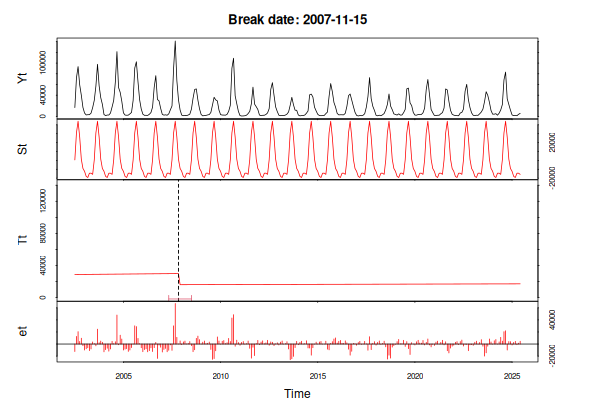
\includegraphics[scale=0.45]
    {figures/plot_bfast_brazil_year_month_AQUA_M-T.png}
    \caption{BFAST identified a break in the trend component of the AQUA M-T
    fire foci times series.}
  \end{figure}
\end{frame}

\begin{frame}[label=bfast_aqua]
  \frametitle{AQUA M-T annual top values trend after BFast breaks}
  \begin{figure}
    \centering
    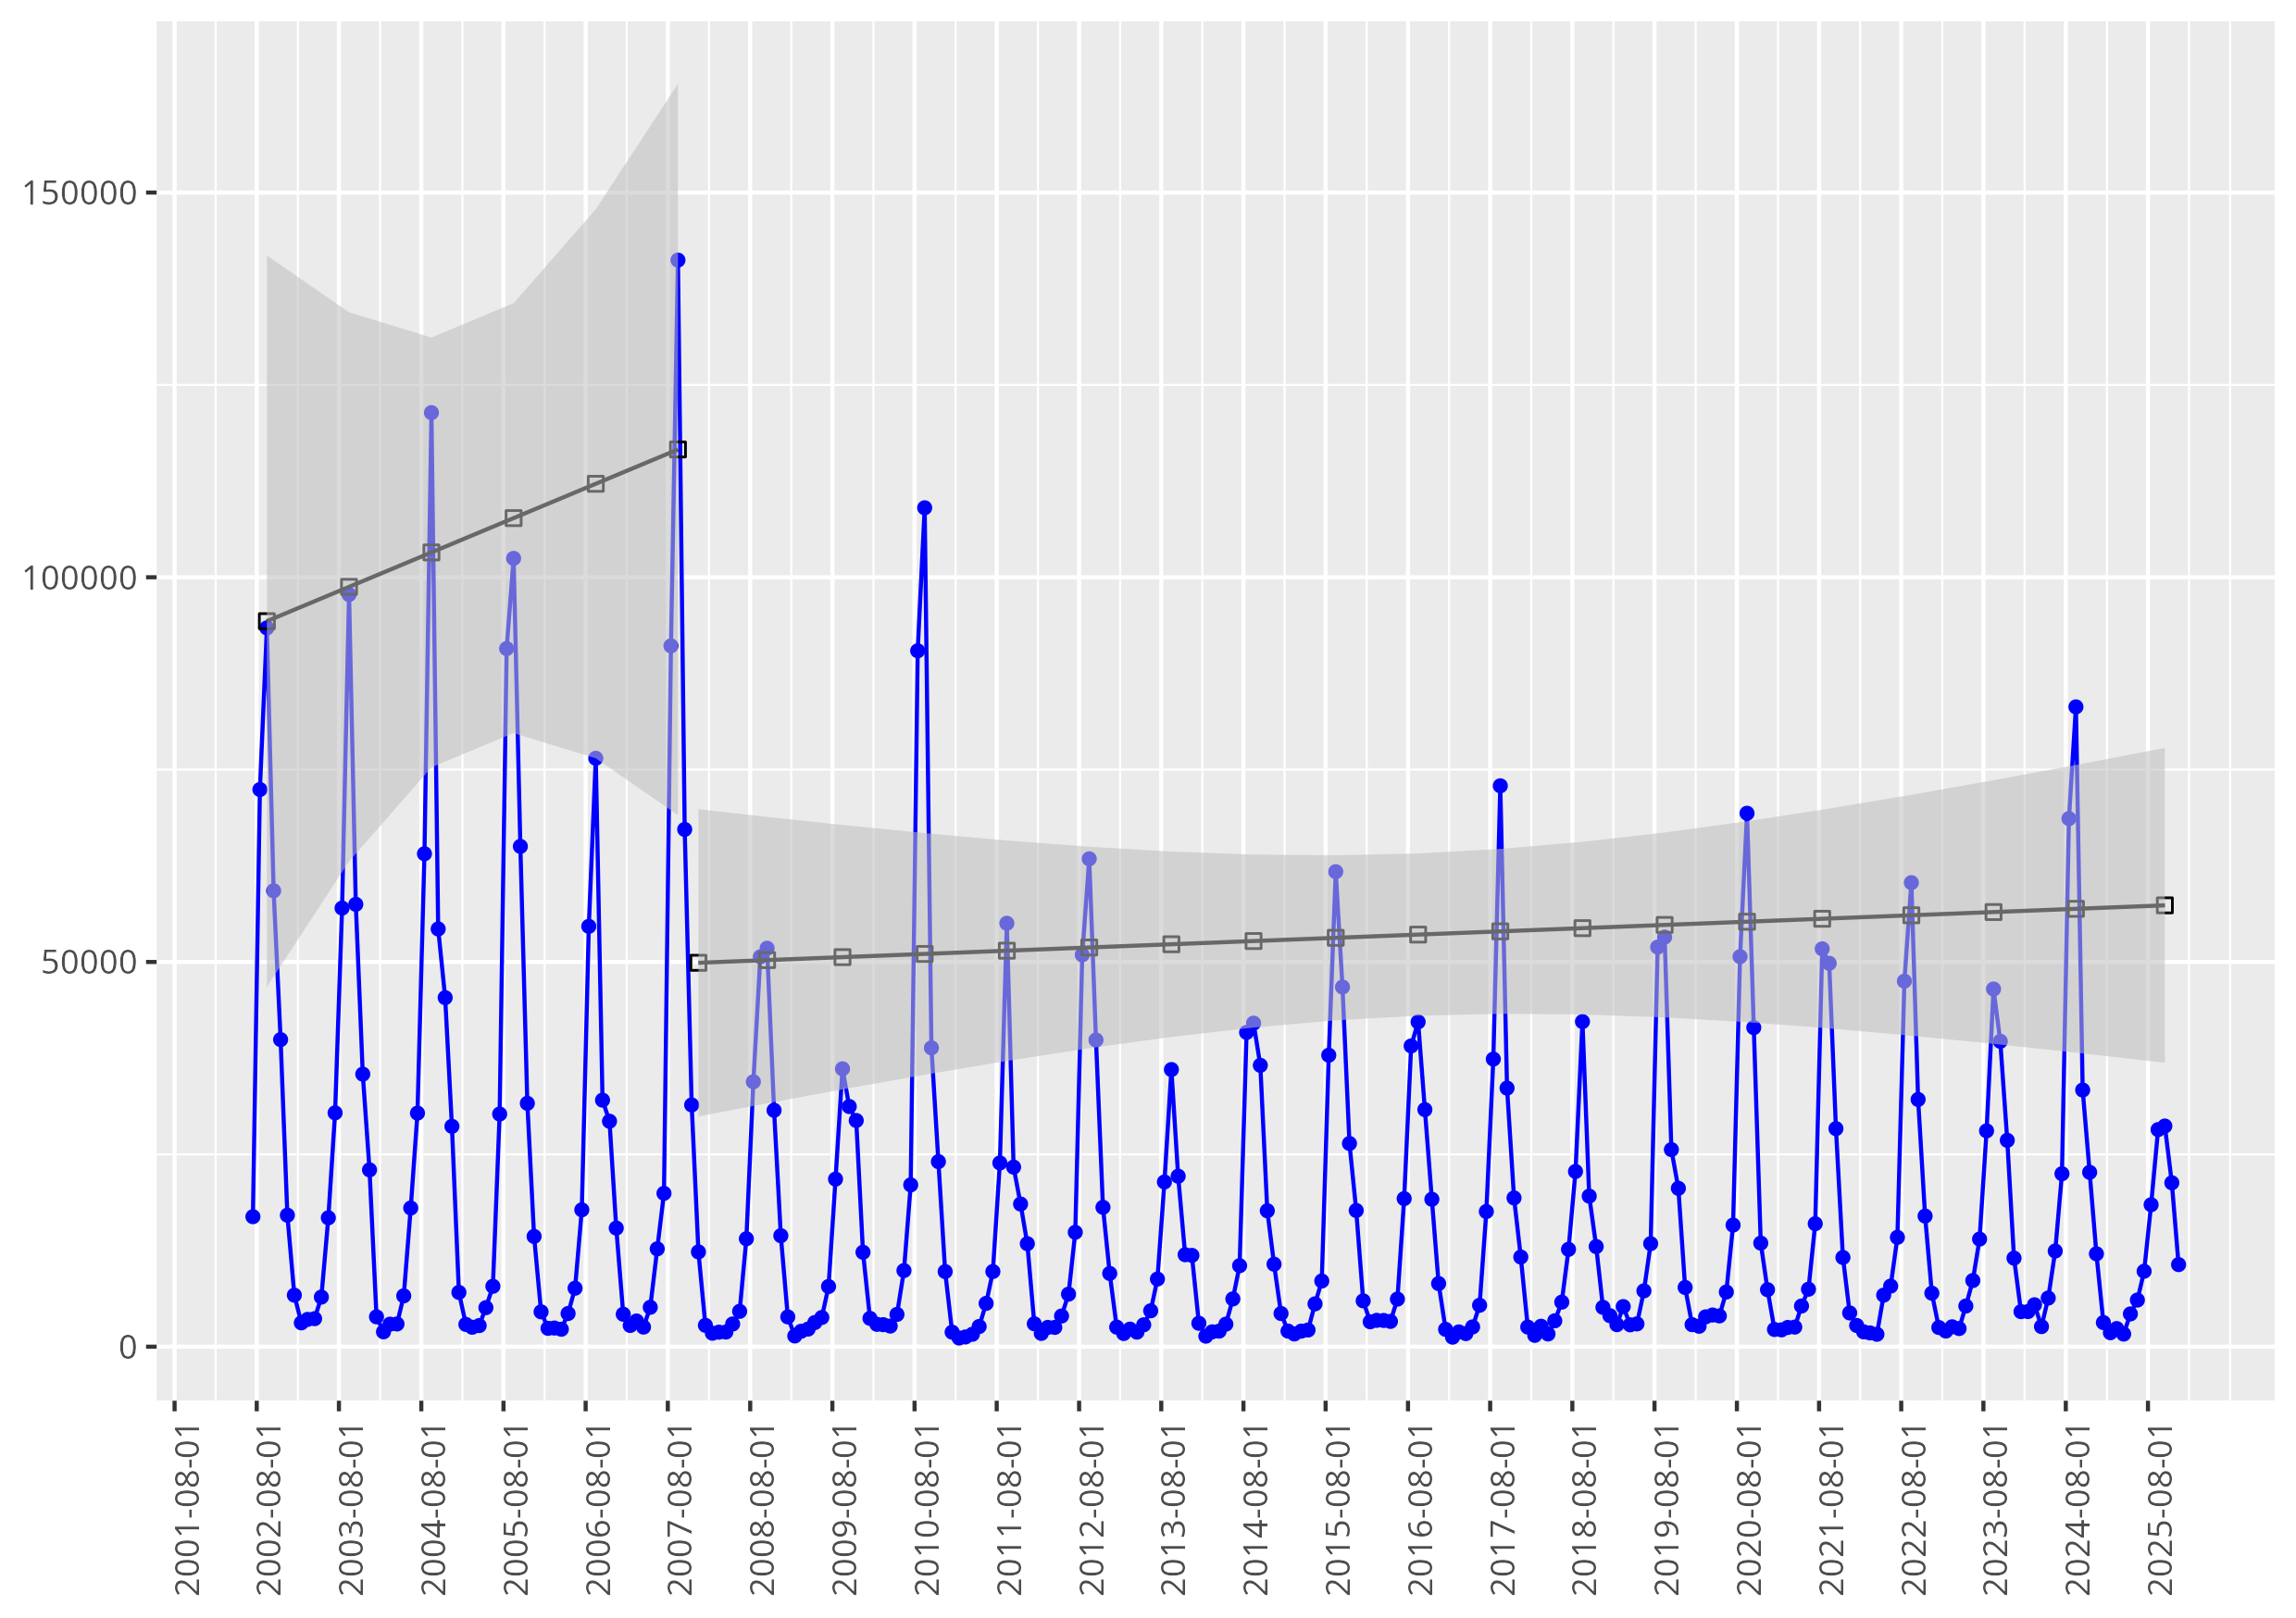
\includegraphics[scale=0.45]
    {figures/plot_bfast_split_brazil_year_month_AQUA_M-T.png}
    \caption{Annual-peak trends are positive before and after the break. (in
    contrast to no break~\hyperlink{lm_peak}{\beamergotobutton{}}).}
  \end{figure}
\end{frame}

\begin{frame}
  \frametitle{Time series breaks (BFast) NOAA-12}
  \begin{figure}
    \centering
    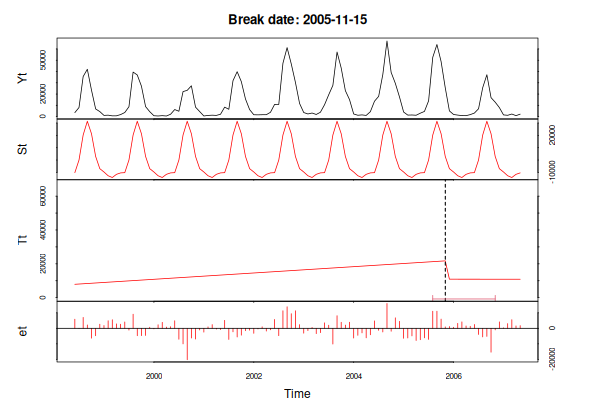
\includegraphics[scale=0.45]
    {figures/plot_bfast_brazil_year_month_NOAA-12.png}
    \caption{BFAST didn't find a break in NOAA-12 fire foci time seires.}
  \end{figure}
\end{frame}

\begin{frame}[label=bfast_noaa]
  \frametitle{NOAA-12 annual top values trend after BFast breaks}
  \begin{figure}
    \centering
    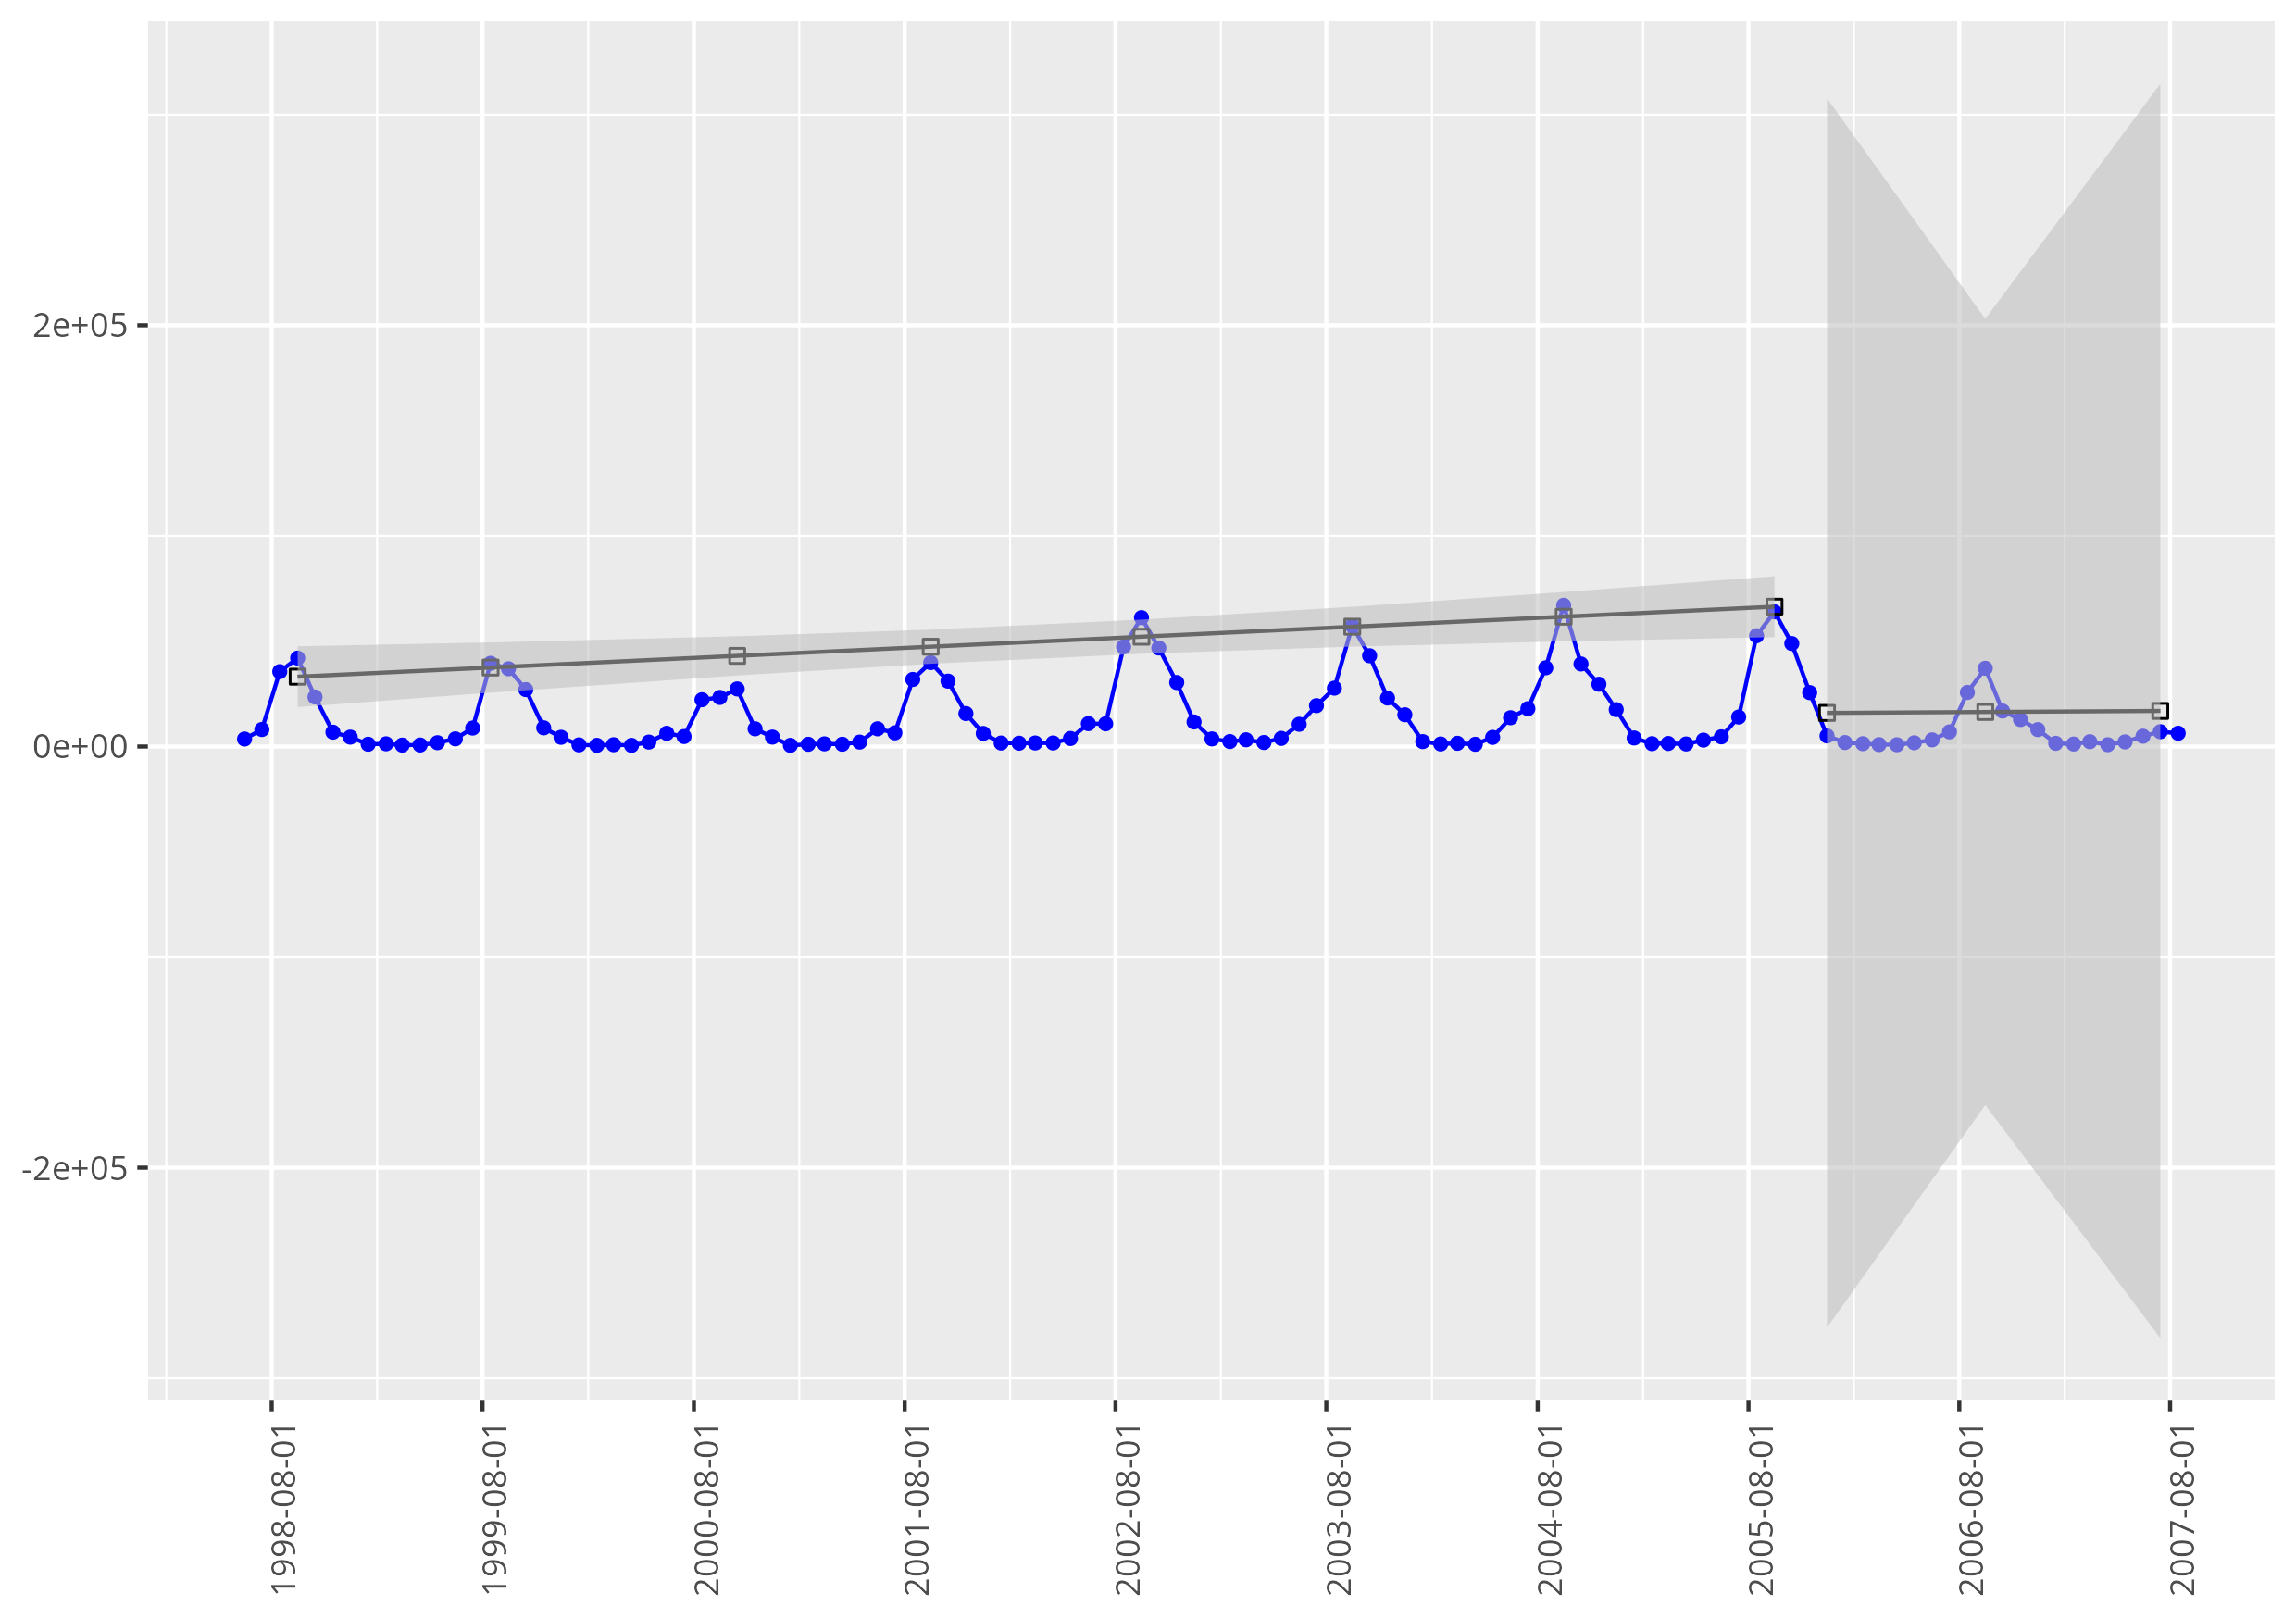
\includegraphics[scale=0.45]
    {figures/plot_bfast_split_brazil_year_month_NOAA-12.png}
    \caption{The annual-peak trend is slightly positive before break and
    neutral after it. (in contrast to no
    break~\hyperlink{lm_peak}{\beamergotobutton{}}).}
  \end{figure}
\end{frame}

\begin{frame}
  \frametitle{Time series breaks (BFast) NPP-375-PM}
  \begin{figure}
    \centering
    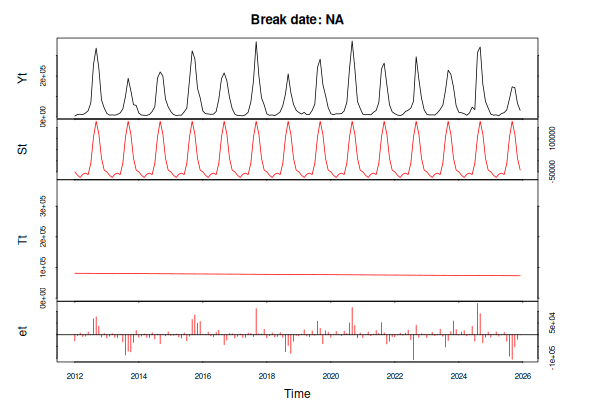
\includegraphics[scale=0.45]
    {figures/plot_bfast_brazil_year_month_NPP-375-PM.png}
    \caption{BFAST didn't find a break in NPP-375-PM fire foci time seires.}
  \end{figure}
\end{frame}

\begin{frame}
  \frametitle{Time series breaks (BFast) NPP-375-PM}
  \begin{figure}
    \centering
    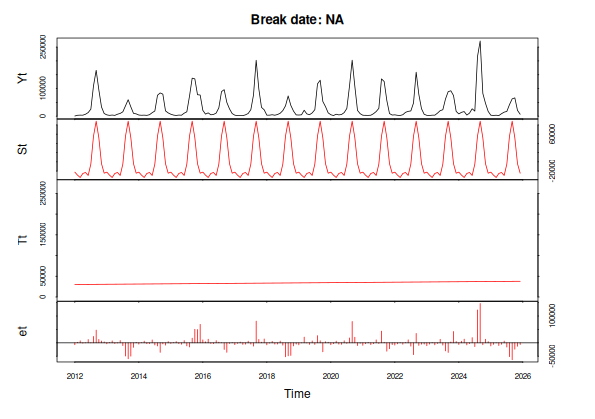
\includegraphics[scale=0.45]
    {figures/plot_bfast_brazil_year_month_NPP-375D.png}
    \caption{BFAST didn't find a break in NPP-375D fire foci time seires.}
  \end{figure}
\end{frame}
